\documentclass[10pt,letterpaper,english]{article}
\usepackage{mathpazo}
\usepackage[hmargin=2cm,vmargin=2cm]{geometry}
\usepackage{graphicx}
\usepackage{marvosym}
\usepackage{subfigure}
\usepackage{amsmath}
\usepackage{multicol}
\usepackage{float}
\usepackage{booktabs}
\usepackage{enumerate}
\usepackage{dingbat}
\usepackage{tikz-timing}[2009/05/15]
\usepackage{amsthm}% http://ctan.org/pkg/amsthm
\renewcommand*\thesection{\arabic{section}.0}
\usepackage{pdfpages}
\usepackage{calc}
\usetikzlibrary{circuits.logic.US,calc, positioning}
\usepackage{tikz-timing}
%\renewcommand{\familydefault}{\sfdefault}
%\usepackage{helvet}
\usepackage{babel}
\usepackage{fancyhdr}
\pagestyle{empty}
\usepackage[compact]{titlesec}
\titlespacing{\section}{0pt}{2ex}{1ex}
\titlespacing{\subsection}{0pt}{2ex}{1ex}
\titlespacing{\subsubsection}{0pt}{0.4ex}{0ex}


  \hyphenpenalty=500000
  \tolerance=1000

% indentsection style, used for sections that aren't already in lists
% that need indentation to the level of all text in the document
\newenvironment{indentsection}[1]{\begin{list}{}%
{\setlength{\leftmargin}{#1}}%
\item[]%
}{\end{list}}

% opposite of above; bump a section back toward the left margin
\newenvironment{unindentsection}[1]{\begin{list}{}%
{\setlength{\leftmargin}{-0.5#1}}%
\item[]%
}{\end{list}}

% format two pieces of text, one left aligned and one right aligned
\newcommand{\headerrow}[2]{\begin{tabular*}{\linewidth}[t]{l@{\extracolsep{\fill}}r}
#1 &
#2 \\
\end{tabular*}}

\thispagestyle{fancy}
\renewcommand{\headrulewidth}{0pt}
\rfoot{HSV, DJS, RDN}    
\cfoot{}
\begin{document}

\textsc{op-amps}\\
% refer to here zebu.uoregon.edu/~rayfrey/431/notes9.pdf
Virtual short: V+ = V-\\
There's a PDF in the comment, read it and grab the relevant parts.

\begin{multicols}{2}
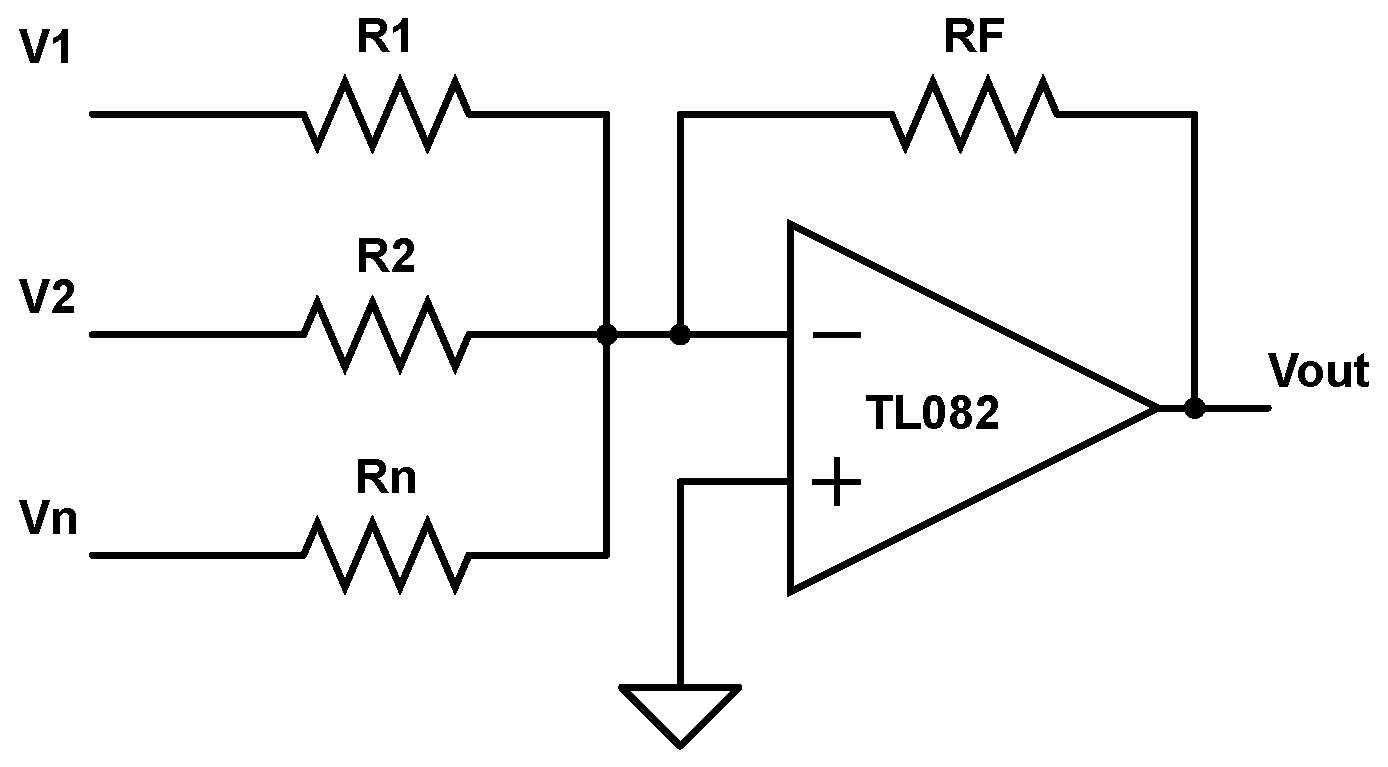
\includegraphics[scale=0.2]{opamp-1.eps}
\begin{align*}
V_{out} = -\left(\frac{R_F}{R_1}\cdot V_1 + \frac{R_F}{R_2}\cdot V_2 \cdots + \frac{R_F}{R_n}\cdot V_n\right)
\end{align*}
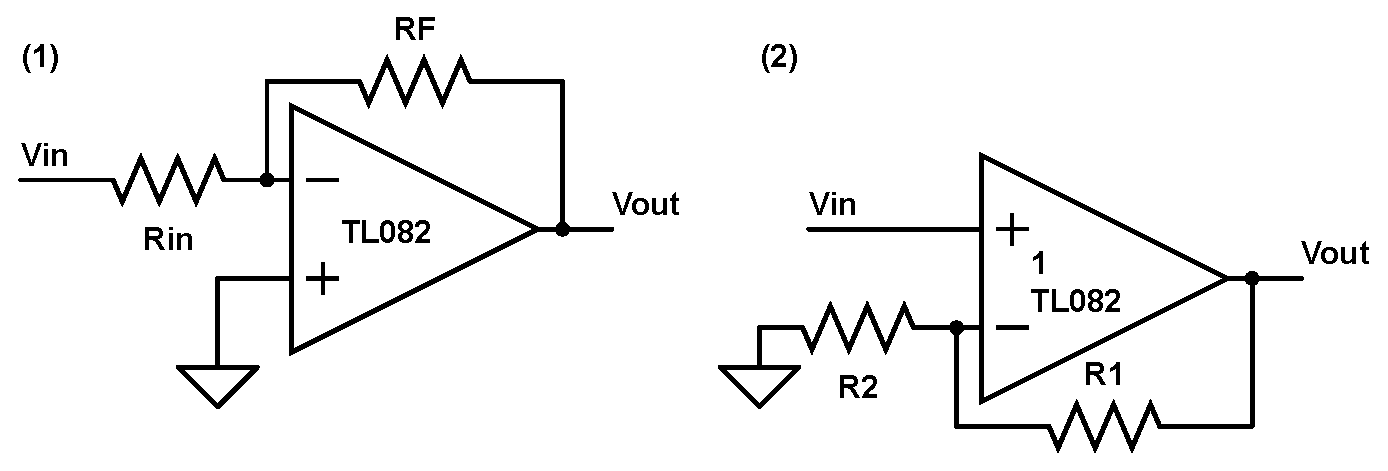
\includegraphics[scale=0.4]{opamp-2.eps}
\begin{align*}
V_{out} = -\frac{R_F}{R_{in}}\cdot V_{in} \tag*{(1) Inverting}\\
V_{out} = \left(1 + \frac{R_1}{R_2}\right)\cdot V_{in} \tag*{(2) Non-inverting}\\
\end{align*}
\end{multicols}


\begin{multicols}{2}
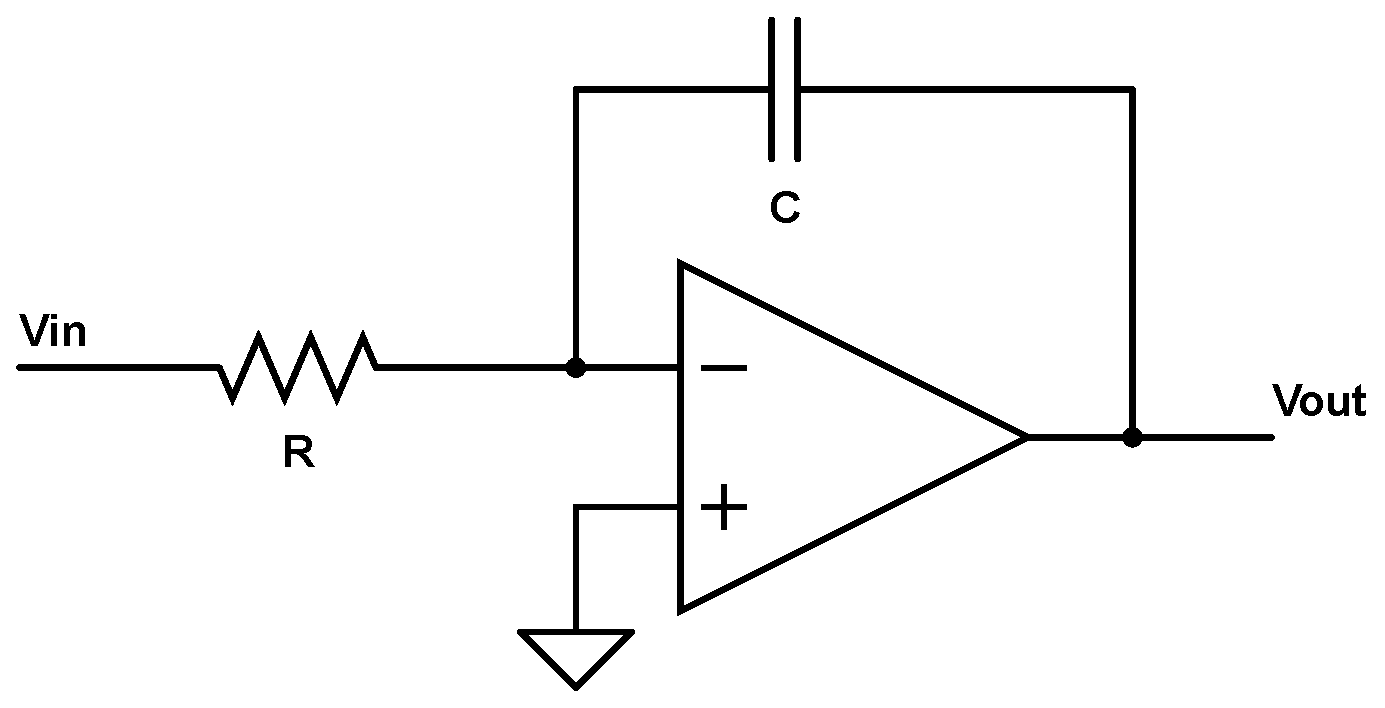
\includegraphics[scale=0.2]{opamp-integrator.eps}
\begin{align*}
V_{out} = -\int_0^t \frac{V_{in}}{RC} \,dt; \frac{V_{out}}{V_{in}} = \frac{-1}{j \omega RC} \tag*{Integrator / Low-pass}\\
\end{align*}
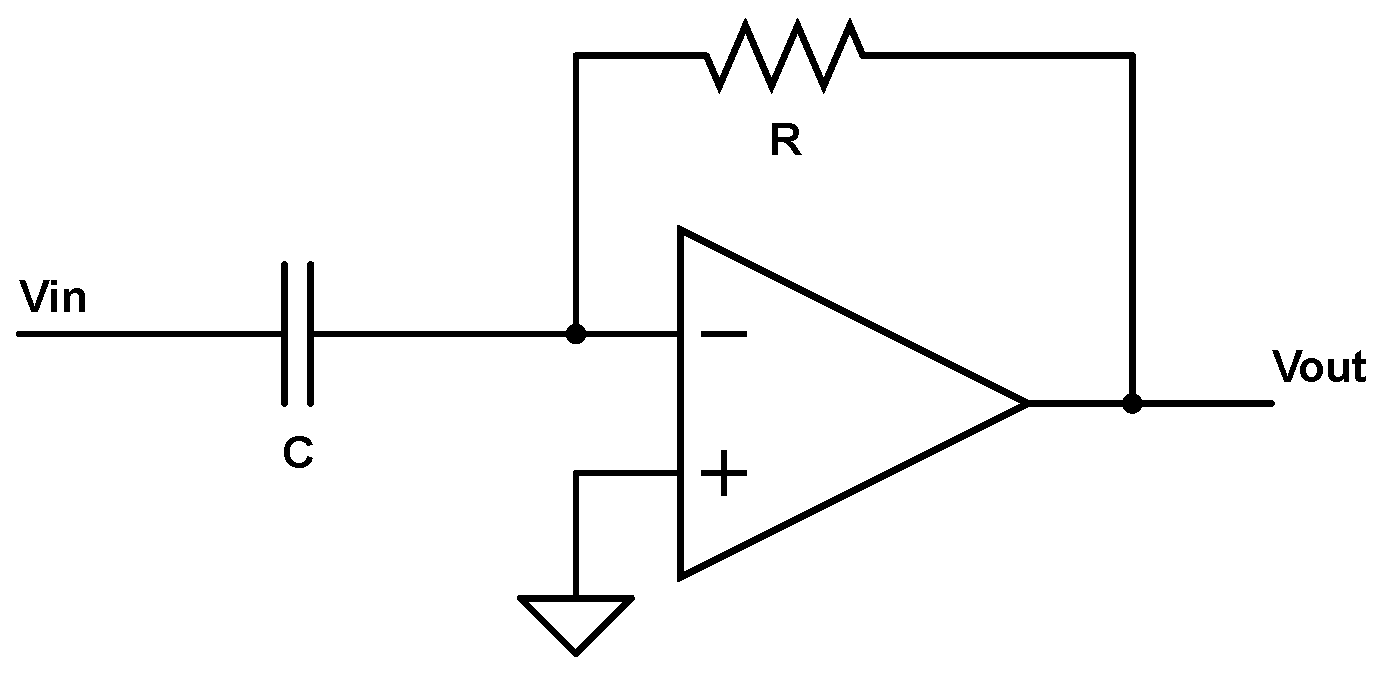
\includegraphics[scale=0.2]{opamp-differentiator.eps}
\begin{align*}
V_{out} = -RC \frac{\,dV_{in}}{\,dt} \tag*{Differentiator / High-pass}\\
\end{align*}
\end{multicols}


\textsc{mosfets}\\

\begin{multicols}{2}
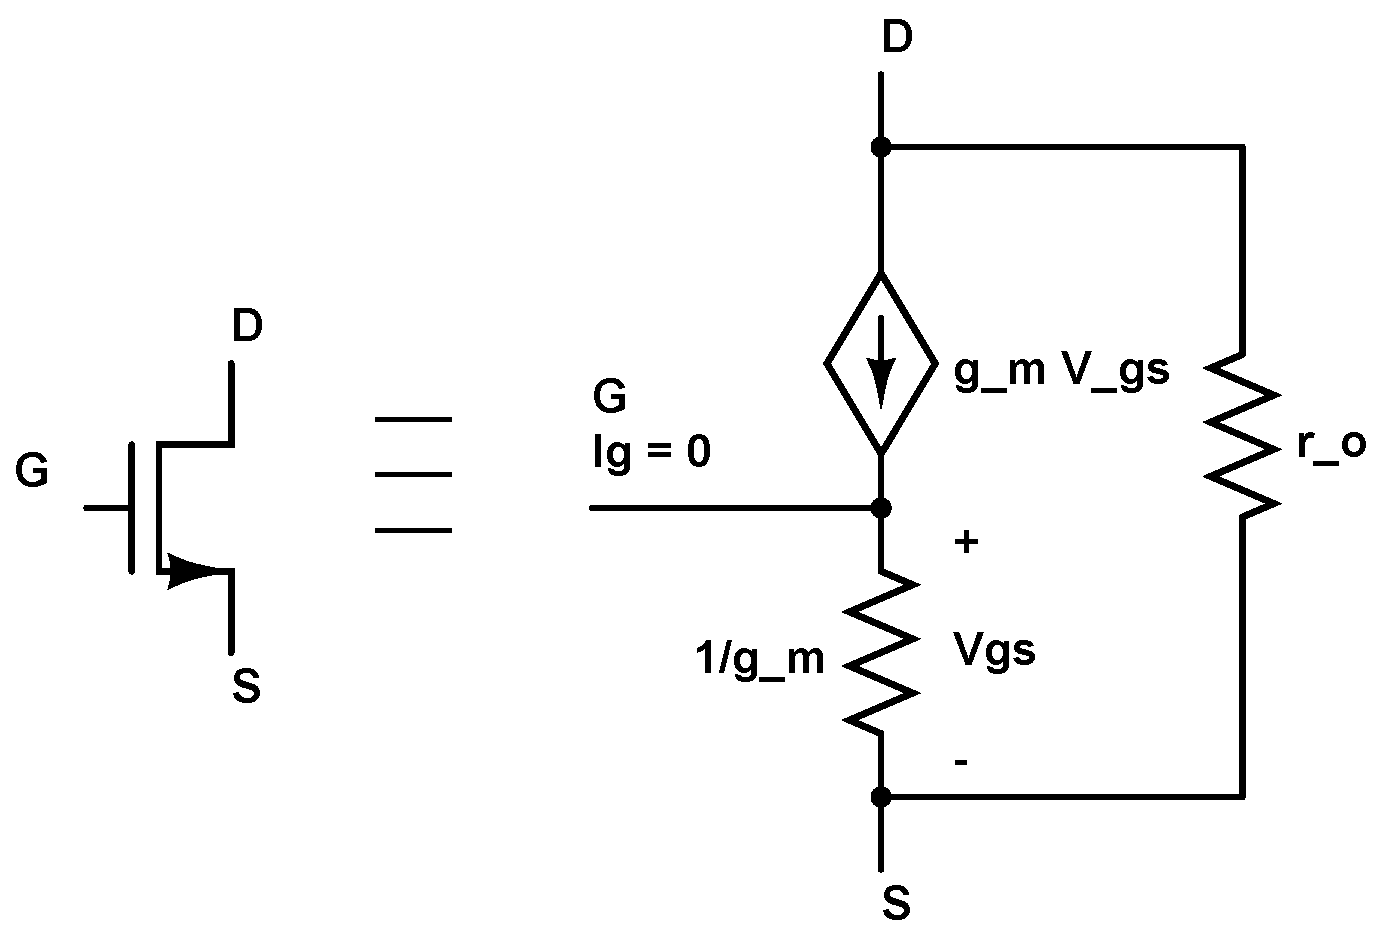
\includegraphics[scale=0.24]{mosfet-t-model.eps}
\begin{align*}
\tag*{Mosfet T-model}\\
\end{align*}
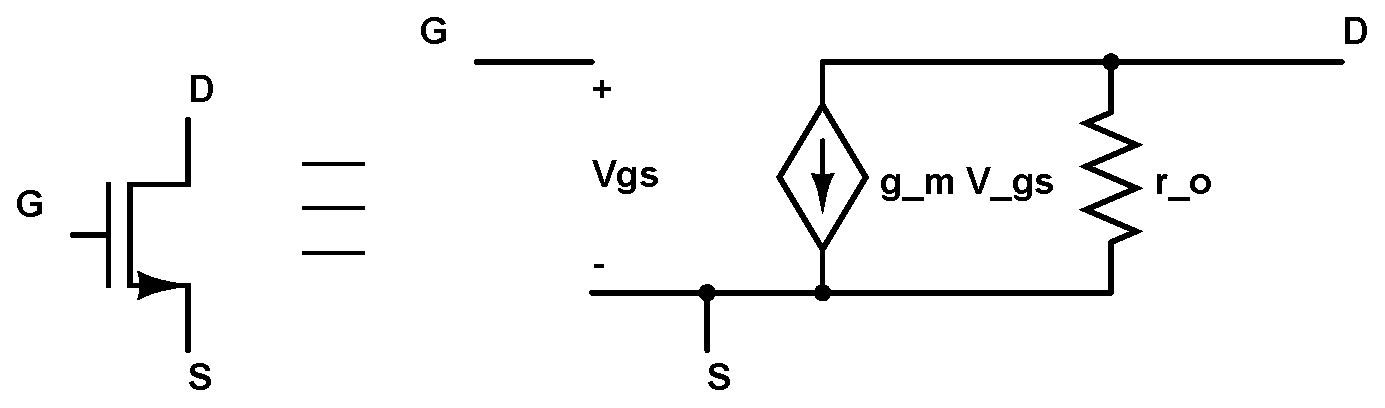
\includegraphics[scale=0.4]{mosfet-hybrid-pi.eps}
\vspace{2mm}
\begin{align*}
A_v = \frac{-g_mr_{out}}{(1 + g_mR_S)} \tag*{Mosfet hybrid pi model}\\
\end{align*}
\end{multicols}

\begin{multicols}{2}
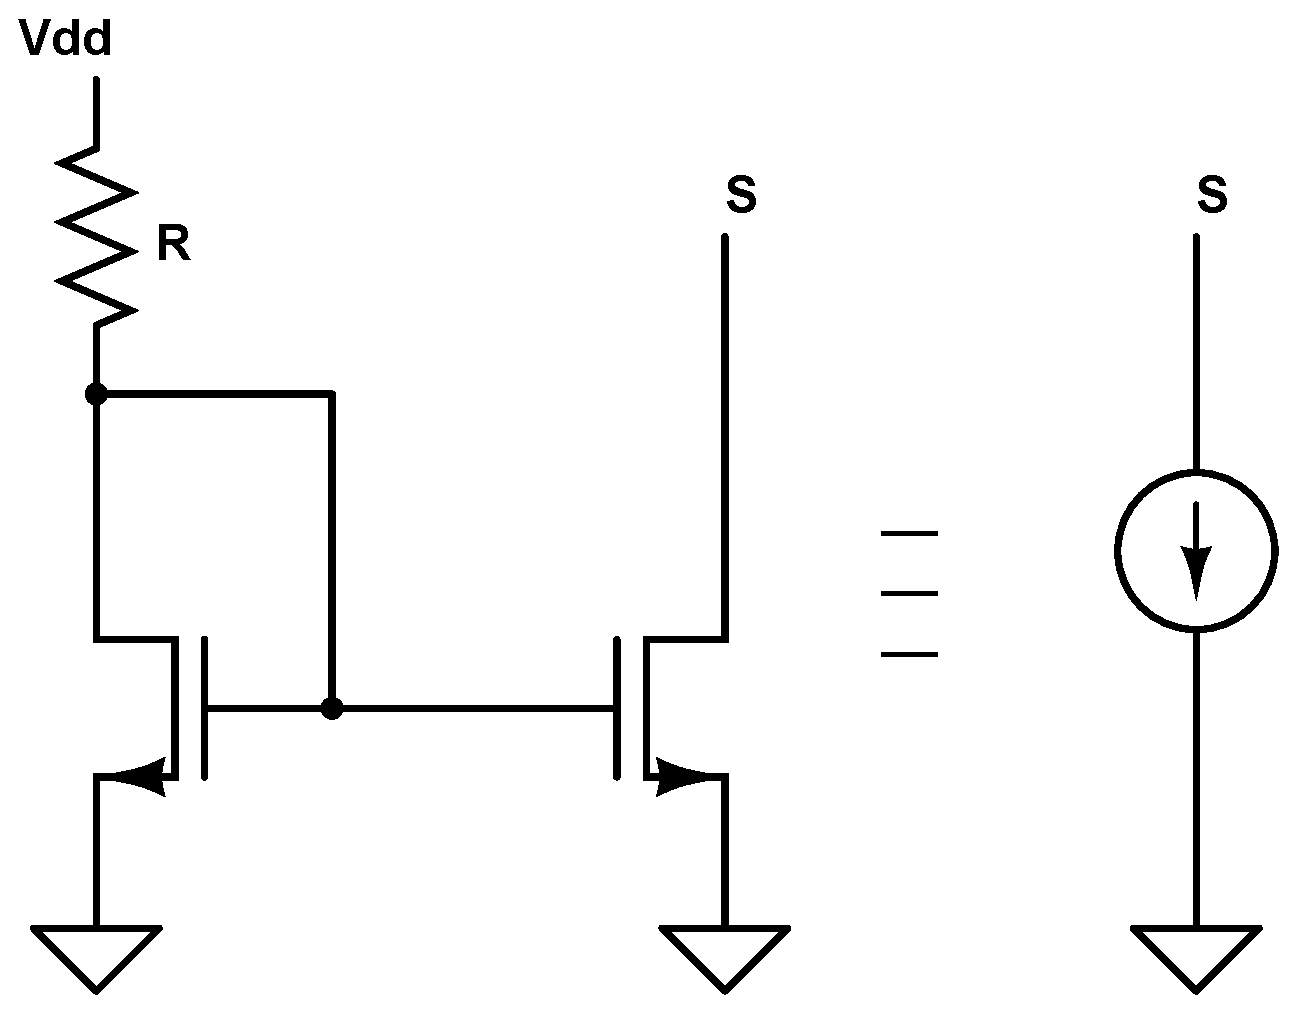
\includegraphics[scale=0.2]{mosfet-current-mirror.eps}
\begin{align*}
I_{current\ source}&= \frac{W_2/L_2}{W_1/L_1}\cdot I_{REF} \tag*{MOSFET current mirror circuit}\nonumber\\
\end{align*}
\end{multicols}

\textsc{MOSFETs}\\
\begin{align}
g_m& = \sqrt{2\mu_n \cdot C_{ox} \cdot I_d} = \sqrt{2I_D\cdot K}\nonumber
\end{align}
High input impedance ($R\rightarrow \infty$)



\begin{multicols}{2}
\textsc{BJTs}
\begin{flalign}
I_C&=I_S\cdot e^{\frac{V_{BE}}{V_T}}\nonumber&\\
I_C&=\beta \cdot I_B, I_C = \alpha I_E\nonumber&\\
\alpha&=\frac{\beta}{\beta + 1}\nonumber&\\
g_m& = \frac{I_c}{V_t}\nonumber = \frac{\beta}{r_\pi}&\\
I_E&= I_C + I_B\nonumber&\\
r_\pi&= \frac{V_T}{I_B}, r_0 = \frac{|V_A|}{I_C}\nonumber&
\end{flalign}
Common Collector Equations (BJT):
\begin{flalign}
A_i &= \beta + 1\nonumber&\\
A_v &=\frac{g_mR_E}{g_mR_E+1} \approx 1\nonumber&\\
r_{in} &= r_\pi+ \left(\beta + 1\right)R_E \approx \beta R_E\nonumber&\\
 r_{out} &= R_E \big|\big| \left(\frac{r_\pi + R_{source}}{\beta + 1}\right) \approx \frac{1}{g_m} + \frac{R_{source}}{\beta}\nonumber&
\end{flalign}
Common Emitter Equations (BJT):
\begin{flalign}
A_i &= \beta&\nonumber\\
A_v &= -\frac{\beta R_C}{r_\pi + \left(\beta + 1\right)R_E}=-\frac{g_mr_\pi R_C}{r_\pi + \left(g_mr_\pi + 1\right)R_E}&\nonumber\\
r_{in} &= r_\pi + \left(\beta + 1\right)R_E\nonumber&\\
r_{out} &= R_C\nonumber&
\end{flalign}
Shockley Diode Eqn (Forward Biased):
\begin{flalign}
I&= I_S\left(e^{\frac{V_D}{\left(nV_t\right)}} - 1\right)\nonumber
\end{flalign}
Zener Diode Voltage Drop:
\begin{flalign}
V_{Z} &= V_{Z0} + i_Zr_Z\nonumber
\end{flalign}
Mosfet Equations
\begin{flalign}
g_m&=\left.\frac{\partial i_D}{\partial v_{GS}} \right|_{V_{GS}} = K\left(V_{GS} - V_t\right)\nonumber
\end{flalign}
\end{multicols}
\end{document}
